\renewcommand{\thetheorem}{19.\arabic{theorem}}
\setcounter{theorem}{0}
\setcounter{chapter}{18} % Chapter 19
% ---------------------------------------------------------------------------
% Provenance of the prose in this file.
%   % Extractor: <model>   the block below was transcribed from Prof. Biran's
%                          handwritten notes by that model
%   % Creator:   <model>   the block below was written by that model and has no
%                          counterpart in the notes
% A tag holds until the next tag.
% ---------------------------------------------------------------------------

\chapter{Miscellaneous Topics and Motivation}

% Extractor: Gemini 3.1 Pro

\section{Geometric Motivation: Why Abstraction Matters}

It is a common temptation to simply identify every $n$-dimensional vector space over $K$ with the standard coordinate space $K^n$. However, while they are algebraically isomorphic for any fixed parameter, they may not be \qt{continuously} isomorphic when the vector spaces depend dynamically on parameters.

\subsection{The Möbius Vector Bundle}

\begin{definition}[A Continuous Family of Subspaces]
  \label{def:mobius_family}
  Let $S \subseteq \mathbb{C}$ be the unit circle defined by $S = \{e^{i\theta} \mid \theta \in [0, 2\pi]\}$. For each $z = e^{i\theta} \in S$, we define a 1-dimensional subspace $L_z \subseteq \mathbb{R}^2$ as follows:
  \[ L_z := \Sp \left( \left( \cos\tfrac{\theta}{2}, \, \sin\tfrac{\theta}{2} \right) \right). \]
  The inner parentheses are those of the vector: $L_z$ is the span of the \emph{single} vector $(\cos\frac{\theta}{2}, \sin\frac{\theta}{2}) \in \mathbb{R}^2$, not of the two scalars.
\end{definition}

Notice a topological anomaly: $z=1$ corresponds to both $\theta=0$ and $\theta=2\pi$.
In the first case ($\theta=0$), the spanning vector is $(1,0)$, so $L_1 = \Sp\big((1,0)\big)$.
In the second case ($\theta=2\pi$), the spanning vector is $(-1,0)$, which gives the exact same subspace $L_1 = \Sp\big((-1,0)\big)$. The line $L_z$ rotates at exactly half the speed of the point $z$.

\begin{center}
  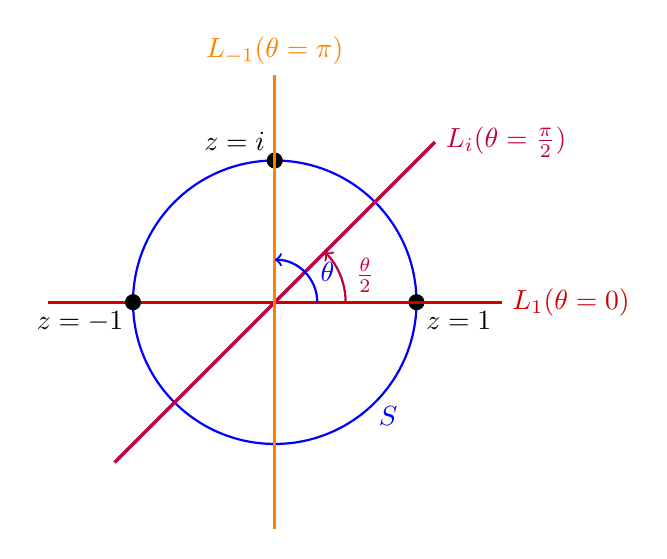
\begin{tikzpicture}[scale=1.8]
    % Background axes
    \draw[gray!40, thin] (-1.5,0) -- (1.5,0);
    \draw[gray!40, thin] (0,-1.5) -- (0,1.5);

    % Unit circle S
    \draw[thick, blue] (0,0) circle (1);
    \node[blue] at (0.8, -0.8) {$S$};

    % theta = 0
    \filldraw[black] (1,0) circle (1.5pt) node[below right] {$z=1$};
    \draw[very thick, red!80!black] (-1.6,0) -- (1.6,0) node[right] {$L_1 (\theta=0)$};

    % theta = pi/2
    \filldraw[black] (0,1) circle (1.5pt) node[above left] {$z=i$};
    \draw[very thick, purple] (-1.13,-1.13) -- (1.13,1.13) node[right] {$L_i (\theta=\frac{\pi}{2})$};

    % theta = pi
    \filldraw[black] (-1,0) circle (1.5pt) node[below left] {$z=-1$};
    \draw[very thick, orange] (0,-1.6) -- (0,1.6) node[above] {$L_{-1} (\theta=\pi)$};

    % Arcs showing the half-speed rotation
    \draw[->, blue, thick] (0.3,0) arc (0:90:0.3) node[midway, right=2pt] {$\theta$};
    \draw[->, purple, thick] (0.5,0) arc (0:45:0.5) node[midway, right=2pt] {$\frac{\theta}{2}$};
  \end{tikzpicture}
\end{center}

\begin{proposition}[Non-triviality of the Möbius Bundle]
  \label{prop:mobius_nontrivial}
  There does not exist a family of linear isomorphisms $T_z \colon L_z \to \mathbb{R}$ that depends continuously on the parameter $z \in S$.
\end{proposition}

\begin{proof}[Proof Sketch]
  Consider the disjoint union of all these lines parameterized by $z$, which forms a space $M = \{ (z, v) \mid z \in S, v \in L_z \}$. Topologically, this forms a vector bundle over $S^1$ known as the Möbius strip.

  If such a continuous family of isomorphisms $T_z$ existed, it would allow us to construct a global homeomorphism $\Phi \colon M \to S \times \mathbb{R}$. Removing the zero-section (the center circle where $v=0$) from both spaces would imply that $M \setminus \{0\} \cong S \times (\mathbb{R} \setminus \{0\})$.

  However, $S \times (\mathbb{R} \setminus \{0\})$ consists of two disconnected cylinders, an \qt{upper} and a \qt{lower} half. In contrast, if you cut a Möbius strip down its centre line, it remains a single connected piece. This topological contradiction demonstrates that we cannot consistently and continuously identify all $L_z$ with $\mathbb{R}$. Abstraction is therefore necessary to handle \qt{twisted} families of spaces.
% Extractor: Opus 5
  This belongs to a branch of mathematics called topology. The conclusion for us is the one the notes draw: each $L_z$ is a one-dimensional vector space over $\mathbb{R}$, so $L_z \cong \mathbb{R}$ for every single $z$, and yet the whole family cannot be identified with $\mathbb{R}$ in a continuous way.
% Extractor: Gemini 3.1 Pro
\end{proof}

\section{Affine Geometry}

In our strict definition of a vector space, there is always a distinguished origin $0$. Affine geometry studies spaces that \qt{look like} vector spaces locally, but have forgotten their origin.

\begin{definition}[Affine Space]
  \label{def:affine_space}
  A subset $X \subseteq V$ is called an \newterm{affine space} if there exists a linear subspace $U \subseteq V$ and a translation vector $x_0 \in V$ such that $X = x_0 + U$.

  We say that $X$ is modeled on the subspace $U$, and we write the \newterm{direction space} as $\vec{X} := U$. The elements of $X$ are called \newterm{points}, while the elements of $\vec{X}$ are called \newterm{vectors}.
% Extractor: Opus 5
  The \newterm{dimension} of $X$ is defined as $\dim X := \dim U$.
\end{definition}

\begin{remark}
\label{rem:affine_x0_not_unique}
The point $x_0$ in \cref{def:affine_space} is not uniquely determined by $X$, unless $\dim X = 0$: any point of $X$ will serve. The subspace $U$, on the other hand, \emph{is} uniquely determined by $X$, which is what makes the notation $\vec{X}$ legitimate. This is left as an exercise.
\end{remark}

% Creator: Opus 5
% The uniqueness of U is what makes the notation \vec{X} of the definition
% above well defined, so the chapter cannot really do without it. The notes
% leave it to the reader and the transcript repeated that; it is now an
% exercise proper, with its solution at the end of the chapter.
\begin{exercise}[The Direction Space is Determined by the Affine Space]
\label{exc:direction_space_unique}
Let $X \subseteq V$ be an affine space. Show that the subspace $U$ of \cref{def:affine_space} is uniquely determined by $X$, and that any point of $X$ may be taken as the base point $x_0$. Deduce that $x_0$ is unique precisely when $\dim X = 0$.
\exinfo{This exercise is taken from Prof.~Biran's handwritten lecture notes.}
\exsol{sol:direction_space_unique}
\end{exercise}

% Extractor: Gemini 3.1 Pro
\begin{proposition}[Algebra of Affine Spaces]
  \label{prop:affine_algebra}
  Let $X$ be an affine space modeled on $\vec{X}$. Then:
  \begin{enumerate}[label=\textbf{(\alph*)}]
    \item We cannot inherently add two points $p, q \in X$, as $p+q \notin X$ in general.
    \item We can translate a point $p \in X$ by a vector $v \in \vec{X}$ to obtain a new point $p+v \in X$.
    \item For any two points $p, q \in X$, their difference defines a unique vector $\vec{pq} := q - p \in \vec{X}$.
  \end{enumerate}
\end{proposition}

% Extractor: Opus 5
\begin{proof}
For \textbf{(b)}, write $p = x_0 + u$ with $u \in \vec{X}$. Then $p + v = x_0 + (u + v) \in x_0 + \vec{X} = X$, since $u + v \in \vec{X}$. For \textbf{(c)}, write $p = x_0 + u$ and $q = x_0 + v$ with $u, v \in \vec{X}$; then $q - p = v - u \in \vec{X}$. Statement \textbf{(a)} is the observation that on $X$ there is no longer a zero: an affine space has forgotten its origin.
\end{proof}

Note also that the two operations fit together as one expects: $p + \vec{pq} = q$ for all $p, q \in X$.

\begin{example}[Affine Spaces]
\label{ex:affine_spaces}
\begin{enumerate}[label=\textbf{(\alph*)}]
    \item An \newterm{affine point} is an affine space $X = \{x\} \subseteq V$ with $\vec{X} = \{0\}$, so $\dim X = 0$.
    \item An \newterm{affine line}: let $x, y \in V$ be distinct and put $v := \vec{xy}$. Then
    \[
    \ell_{xy} := \{x + t v \mid t \in K\}
    \]
    is an affine line, modeled on the one-dimensional subspace $\Sp(v)$.
    \item In the same way one considers affine $2$-dimensional planes, and generally affine $k$-dimensional planes, modeled on $k$-dimensional subspaces.
    \item Let $A \in \M_{m \times n}(K)$ and $b \in K^m$, and let $x_0 \in K^n$ be a solution of $Ax = b$. Then, by \cref{cor:non_homogeneous_solutions},
    \[
    \underbrace{\Sol(A, b)}_{\text{affine space}} = x_0 + \underbrace{\Sol(A, 0)}_{\text{vector space}},
    \]
    so the solution set of an inhomogeneous linear system is exactly an affine space modeled on the solution space of the associated homogeneous system.
\end{enumerate}
\end{example}

\begin{remark}
One can go further and define \newterm{affine maps} $f \colon X \to Y$ between affine spaces, and, given an affine space $X$ and a subspace $U \subseteq \vec{X}$, a new affine space $X/U$ modeled on $\vec{X}/U$.
\end{remark}

\begin{definition}[Parallel Affine Spaces]
\label{def:affine_parallel}
Let $X, Y \subseteq V$ be affine spaces. We say that $X$ and $Y$ are \newterm{parallel}, written $X \parallel Y$, if $\vec{X} = \vec{Y}$; equivalently, if $X = p + U$ and $Y = q + U$ for one and the same subspace $U$. We say that $X$ is \newterm{weakly parallel} to $Y$ if $\vec{X} \subseteq \vec{Y}$.
\end{definition}

\begin{importantremark}[Ratios of Vectors on a Line]
\label{rem:ratio_of_vectors}
If $L$ is a \emph{one-dimensional} vector space over $K$, then vectors in $L$ can be divided by one another. Indeed, let $u, v \in L$ with $u \neq 0$. Since $\dim L = 1$, the vector $u$ alone is a basis of $L$, so there is a unique scalar $\lambda \in K$ with $v = \lambda \cdot u$, and we define
\[
\frac{v}{u} := \lambda \in K.
\]
Consequently, if $X$ is an affine line and $a, b, c \in X$ with $a \neq b$, then $\vec{ab}$ and $\vec{ac}$ both lie in the one-dimensional space $\vec{X}$ and $\vec{ab} \neq 0$, so the ratio
\[
\frac{\vec{ac}}{\vec{ab}} \in K
\]
is defined. These are proportions, not distances: no notion of length is involved, and none is available, since $K$ need not be $\mathbb{R}$.
\end{importantremark}

% Extractor: Gemini 3.1 Pro

\begin{center}
  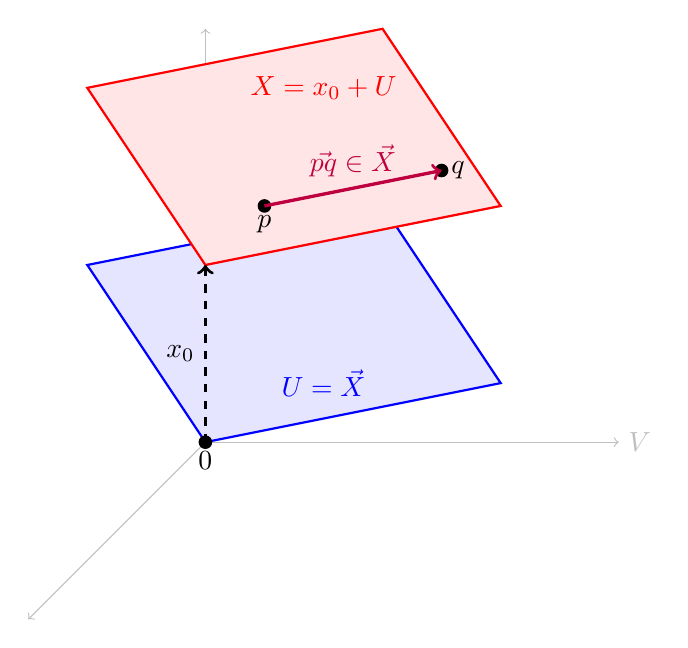
\begin{tikzpicture}[scale=1.5]
    % Axes to imply ambient space V
    \draw[->, gray!50] (0,0) -- (3.5,0) node[right] {$V$};
    \draw[->, gray!50] (0,0) -- (0,3.5);
    \draw[->, gray!50] (0,0) -- (-1.5,-1.5);

    % Subspace U (passing through origin)
    \filldraw[blue!10, draw=blue, thick] (0,0) -- (2.5,0.5) -- (1.5,2) -- (-1,1.5) -- cycle;
    \node[blue] at (1,0.5) {$U = \vec{X}$};

    % Affine space X (displaced)
    \filldraw[red!10, draw=red, thick] (0,1.5) -- (2.5,2.0) -- (1.5,3.5) -- (-1,3.0) -- cycle;
    \node[red] at (1,3) {$X = x_0 + U$};

    % Origin and translation
    \filldraw[black] (0,0) circle (1.5pt) node[below] {$0$};
    \draw[->, very thick, dashed] (0,0) -- (0,1.5) node[midway, left] {$x_0$};

    % Points in X
    \filldraw[black] (0.5, 2.0) circle (1.5pt) node[below] {$p$};
    \filldraw[black] (2.0, 2.3) circle (1.5pt) node[right] {$q$};
    \draw[->, very thick, purple] (0.5, 2.0) -- (2.0, 2.3) node[midway, above] {$\vec{pq} \in \vec{X}$};
  \end{tikzpicture}
\end{center}

% Extractor: Opus 5
\begin{theorem}[Thales' Theorem in Affine Geometry]
  \label{thm:thales_affine}
  Let $V$ be a $3$-dimensional vector space over $K$, and let $H, H', H''$ be three distinct parallel $2$-dimensional affine planes in $V$. Let $\ell_1, \ell_2$ be two affine lines, neither of them weakly parallel to $H$, and put
  \[
  p_1 := H \cap \ell_1, \quad p_1' := H' \cap \ell_1, \quad p_1'' := H'' \cap \ell_1, \qquad p_2 := H \cap \ell_2, \quad p_2' := H' \cap \ell_2, \quad p_2'' := H'' \cap \ell_2.
  \]
  Then
  \[ \frac{\vec{p_1 p_1''}}{\vec{p_1 p_1'}} = \frac{\vec{p_2 p_2''}}{\vec{p_2 p_2'}}. \]
  In other words, this ratio does not depend on the line $\ell$ chosen, but only on the three planes $H, H', H''$.
\end{theorem}

\begin{proof}
Put $U := \vec{H} = \vec{H'} = \vec{H''}$, which is a $2$-dimensional subspace of $V$, the three planes being parallel. Consider the quotient $V/U$ and the projection $\pi \colon V \to V/U$. By \cref{prop:dim_quotient},
\[
\dim V/U = \dim V - \dim U = 3 - 2 = 1,
\]
so $V/U$ is a line, and ratios of its non-zero vectors are defined as in \cref{rem:ratio_of_vectors}.

Both ratios in the statement are defined: $p_1, p_1', p_1''$ lie on the affine line $\ell_1$, whose direction space is one-dimensional, and $\vec{p_1 p_1'} \neq 0$ because $p_1 \in H$ and $p_1' \in H'$ are points of distinct parallel planes. Put
\[
\lambda_1 := \frac{\vec{p_1 p_1''}}{\vec{p_1 p_1'}}, \qquad \lambda_2 := \frac{\vec{p_2 p_2''}}{\vec{p_2 p_2'}},
\]
so that $\vec{p_1 p_1''} = \lambda_1 \vec{p_1 p_1'}$ and $\vec{p_2 p_2''} = \lambda_2 \vec{p_2 p_2'}$. Our task is to show $\lambda_1 = \lambda_2$.

Now $\pi(\vec{p_1 p_1'}) = \pi(\vec{p_2 p_2'})$. Indeed,
\[
\vec{p_1 p_1'} - \vec{p_2 p_2'} = \vec{p_1 p_2} + \vec{p_2' p_1'} \in U,
\]
because $p_1, p_2 \in H$ gives $\vec{p_1 p_2} \in \vec{H} = U$, and $p_2', p_1' \in H'$ gives $\vec{p_2' p_1'} \in \vec{H'} = U$; and $\ker(\pi) = U$ by \cref{prop:quotient_map}. The same argument with $H''$ in place of $H'$ gives $\pi(\vec{p_1 p_1''}) = \pi(\vec{p_2 p_2''})$. Combining, and using the linearity of $\pi$,
\[
\lambda_1 \, \pi(\vec{p_1 p_1'}) = \pi(\lambda_1 \vec{p_1 p_1'}) = \pi(\vec{p_1 p_1''}) = \pi(\vec{p_2 p_2''}) = \pi(\lambda_2 \vec{p_2 p_2'}) = \lambda_2 \, \pi(\vec{p_2 p_2'}) = \lambda_2 \, \pi(\vec{p_1 p_1'}).
\]
Finally, $\pi(\vec{p_1 p_1'}) \neq 0$: otherwise $\vec{p_1 p_1'} \in \ker(\pi) = U$, and since $\vec{p_1 p_1'}$ spans the direction space of $\ell_1$, this would make $\ell_1$ weakly parallel to $H$, which we excluded. Cancelling the non-zero vector $\pi(\vec{p_1 p_1'})$ in the one-dimensional space $V/U$ yields $\lambda_1 = \lambda_2$.
\end{proof}

\begin{remark}
Observe what this proof did \emph{not} use: no coordinates, no lengths, no angles, and no assumption on $K$ beyond its being a field. The whole argument is the observation that collapsing the direction $U$ of the three planes turns them into three points of a line, where the ratio is visible at once. The four points $p_1, p_2, p_1', p_2'$ need not lie in a common plane, and the same goes for $p_1, p_2, p_1'', p_2''$.
\end{remark}

% Extractor: Gemini 3.1 Pro

\begin{center}
  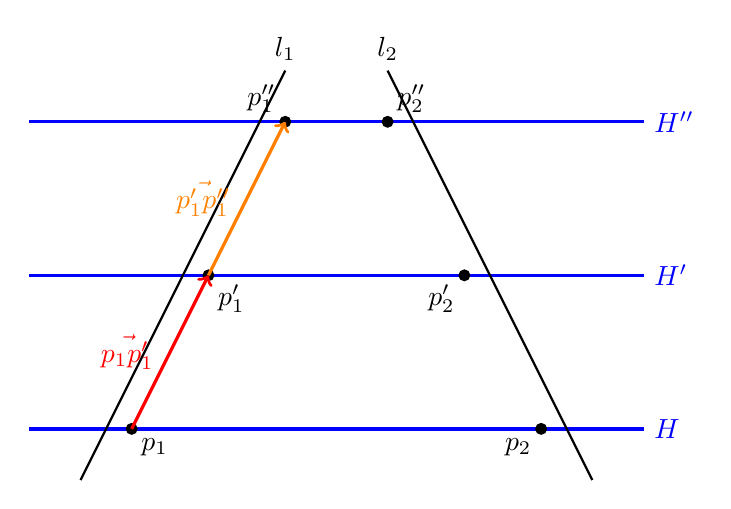
\begin{tikzpicture}[scale=1.3]
    % Parallel planes (represented as lines in 2D projection)
    \draw[very thick, blue] (-1, 3) -- (5, 3) node[right] {$H''$};
    \draw[very thick, blue] (-1, 1.5) -- (5, 1.5) node[right] {$H'$};
    \draw[very thick, blue] (-1, 0) -- (5, 0) node[right] {$H$};

    % Transversal line 1
    \draw[thick, black] (-0.5,-0.5) -- (1.5, 3.5) node[above] {$l_1$};
    \filldraw (0, 0) circle (1.5pt) node[below right] {$p_1$};
    \filldraw (0.75, 1.5) circle (1.5pt) node[below right] {$p_1'$};
    \filldraw (1.5, 3) circle (1.5pt) node[above left] {$p_1''$};

    % Transversal line 2
    \draw[thick, black] (4.5,-0.5) -- (2.5, 3.5) node[above] {$l_2$};
    \filldraw (4, 0) circle (1.5pt) node[below left] {$p_2$};
    \filldraw (3.25, 1.5) circle (1.5pt) node[below left] {$p_2'$};
    \filldraw (2.5, 3) circle (1.5pt) node[above right] {$p_2''$};

    % Vector highlights (corrected)
    \draw[->, very thick, red] (0,0) -- (0.75, 1.5) node[midway, left=2pt] {$\vec{p_1 p_1'}$}; % Vector p1 p1'
    \draw[->, very thick, orange] (0.75, 1.5) -- (1.5, 3) node[midway, left=2pt] {$\vec{p_1' p_1''}$}; % Vector p1' p1''
  \end{tikzpicture}
\end{center}

\section{Introduction to Eigenvalues: Fibonacci Sequences}

\subsection{The Vector Space of Fibonacci Sequences}

Consider the set $\Fib \subseteq \mathbb{R}^\infty$ of all infinite real sequences $(a_0, a_1, a_2, \dots)$ that satisfy the linear recurrence relation $a_n = a_{n-1} + a_{n-2}$ for all $n \ge 2$.

\begin{proposition}[Structure of $\Fib$]
  \label{prop:fibonacci_structure}
  The set $\Fib$ is a 2-dimensional subspace of $\mathbb{R}^\infty$. The evaluation map $F \colon \Fib \to \mathbb{R}^2$ sending a sequence to its first two terms, $(a_n) \mapsto (a_0, a_1)$, is a linear isomorphism.
\end{proposition}

% Creator: Opus 5
% Neither the notes nor the transcript prove this, although the eigenvalue
% computation below uses both halves of it: the isomorphism F to test
% independence, and dim Fib = 2 to conclude that two independent sequences
% form a basis. The proof is four lines.
The notes state this without proof, and the computation at the end of this section uses both of its halves, so we supply one.

\begin{proof}
That $\Fib \subseteq \mathbb{R}^\infty$ is a linear subspace is \cref{ex:fib_subspace}. The map $F$ is linear, since both of its coordinates are, addition and scalar multiplication in $\mathbb{R}^\infty$ being defined entry by entry.

$F$ is injective: if $(a_n) \in \Fib$ has $a_0 = a_1 = 0$, then $a_n = a_{n-1} + a_{n-2}$ gives $a_n = 0$ for every $n \ge 2$ by induction, so the sequence is the zero sequence and $\ker(F) = \{0\}$; now apply \cref{prop:injectivity_kernel} \textbf{(a)}. It is surjective: given $(c_0, c_1) \in \mathbb{R}^2$, set $a_0 := c_0$, $a_1 := c_1$ and define $a_n := a_{n-1} + a_{n-2}$ for $n \ge 2$. This recursion defines a sequence, it satisfies the Fibonacci relation by construction, so it lies in $\Fib$, and $F$ sends it to $(c_0, c_1)$.

Being a bijective linear map, $F$ is an isomorphism by \cref{lem:bijective_is_iso}, and therefore $\dim \Fib = \dim \mathbb{R}^2 = 2$ by \cref{cor:iso_iff_equal_dimension}.
\end{proof}

To find a closed-form formula for the Fibonacci numbers (like Binet's formula), we study the \textbf{shift map} $S \colon \mathbb{R}^\infty \to \mathbb{R}^\infty$ defined by shifting the sequence one position to the left:
\[ S(a_0, a_1, a_2, \dots) := (a_1, a_2, a_3, \dots). \]
Since the shifted sequence also satisfies the Fibonacci recurrence, this map restricts to a linear endomorphism $S' \colon \Fib \to \Fib$.

By utilizing the isomorphism $F$, we can translate the abstract shift operator $S'$ into concrete matrix multiplication on $\mathbb{R}^2$. The sequence $(a_0, a_1)$ shifts to $(a_1, a_2) = (a_1, a_0 + a_1)$, which corresponds to multiplication by the matrix $A = \left(\begin{smallmatrix} 0 & 1 \\ 1 & 1 \end{smallmatrix}\right)$.

\begin{center}
  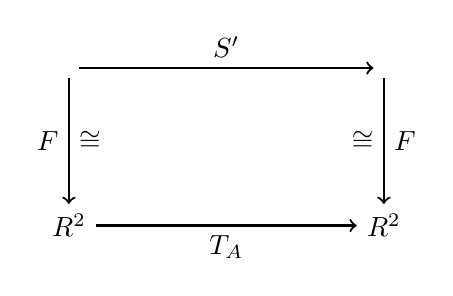
\begin{tikzpicture}[node distance=3cm, auto, thick]
    \node (Fib1) {$\Fib$};
    \node (Fib2) [right of=Fib1, node distance=4cm] {$\Fib$};
    \node (R1) [below of=Fib1, node distance=2cm] {$\mathbb{R}^2$};
    \node (R2) [below of=Fib2, node distance=2cm] {$\mathbb{R}^2$};

    \draw[->] (Fib1) to node {$S'$} (Fib2);
    \draw[->] (Fib1) to node[swap] {$F$} node {$\cong$} (R1);
    \draw[->] (Fib2) to node {$F$} node[swap] {$\cong$} (R2);
    \draw[->] (R1) to node[swap] {$T_A$} (R2);
  \end{tikzpicture}
\end{center}

\subsection{Eigenvalues and Eigenvectors}

The problem of finding a geometric sequence $(1, \lambda, \lambda^2, \dots)$ inside $\Fib$ is equivalent to finding sequences that only scale by $\lambda$ when shifted. That is, we seek vectors $\mathcal{F}$ such that $S'(\mathcal{F}) = \lambda \mathcal{F}$.

\begin{definition}[Eigenvalues and Eigenvectors]
  \label{def:eigenvalue_motivation}
  Let $V$ be a vector space and $T \in \End(V)$. A scalar $\lambda \in K$ is called an \newterm{eigenvalue} of $T$ if there exists a non-zero vector $v \in V$ such that:
  \[ T(v) = \lambda v. \]
  The vector $v$ is called an \newterm{eigenvector} of $T$ associated with the eigenvalue $\lambda$.
\end{definition}

% Extractor: Opus 5
\begin{remark}[Reformulations of the Eigenvalue Condition]
\label{rem:eigenvalue_reformulations}
Unwinding the definition, $\lambda$ is an eigenvalue of $T$ if and only if the linear map $T - \lambda \cdot \id_V \colon V \to V$ has a non-trivial kernel, since $T(v) = \lambda v$ says exactly that $(T - \lambda \id_V)(v) = 0$.

If we assume in addition that $V$ is finite-di\-men\-sional, then by \cref{cor:equal_dim_iso} \textbf{(c)} the last condition is equivalent to
\[
T - \lambda \cdot \id_V \colon V \to V \quad \text{is \emph{not} an isomorphism,}
\]
and, passing to a basis $\mathcal{B}$ of $V$ and writing $n := \dim V$, to
\[
[T]_{\mathcal{B}}^{\mathcal{B}} - \lambda \cdot I_n \in \M_{n \times n}(K) \quad \text{is \emph{not} invertible.}
\]
The last equivalence uses \cref{prop:representation_of_isomorphisms} together with $[\lambda \cdot \id_V]_{\mathcal{B}}^{\mathcal{B}} = \lambda I_n$ from \cref{claim:scaling_map_matrix}. This is the form that will let us actually compute eigenvalues, once we have determinants: it turns the question into a question about a single matrix.
\end{remark}

\begin{proposition}[The Golden Ratio Diagonalises the Shift]
\label{prop:fibonacci_eigenvalues}
Put $\varphi := \frac{1 + \sqrt{5}}{2}$ and $\psi := \frac{1 - \sqrt{5}}{2}$. Then the two geometric sequences
\[
x_{1, \varphi} := (1, \varphi, \varphi^2, \dots), \qquad x_{1, \psi} := (1, \psi, \psi^2, \dots)
\]
belong to $\Fib$, and they form a basis of $\Fib$. Moreover, $\varphi$ and $\psi$ are eigenvalues of the shift $S' \colon \Fib \to \Fib$, with $x_{1,\varphi}$ and $x_{1,\psi}$ as associated eigenvectors.
\end{proposition}

\begin{proof}
A geometric sequence $(1, \lambda, \lambda^2, \dots)$ lies in $\Fib$ precisely when $\lambda^n = \lambda^{n-1} + \lambda^{n-2}$ for all $n \ge 2$, that is, when $\lambda^2 = \lambda + 1$. (The case $n = 2$ already gives that equation, and conversely $\lambda^2 = \lambda + 1$ yields every other case on multiplying by $\lambda^{n-2}$. Note that $\lambda = 0$ is not a solution, so no division by zero is hidden here.) The roots of $\lambda^2 - \lambda - 1$ are exactly $\varphi$ and $\psi$, so both sequences lie in $\Fib$.

They are linearly independent: applying the isomorphism $F$ of \cref{prop:fibonacci_structure} sends them to $(1, \varphi)$ and $(1, \psi)$ in $\mathbb{R}^2$, which are independent because $\varphi \neq \psi$. Since $\dim \Fib = 2$, they form a basis.

Finally, shifting a geometric sequence multiplies it by its ratio:
\[
S'(1, \lambda, \lambda^2, \dots) = (\lambda, \lambda^2, \lambda^3, \dots) = \lambda \cdot (1, \lambda, \lambda^2, \dots),
\]
so $x_{1,\varphi}$ and $x_{1,\psi}$ are eigenvectors of $S'$ with eigenvalues $\varphi$ and $\psi$.
\end{proof}

All that is left in order to recover the closed formula is to express the Fibonacci sequence itself in this basis. The Fibonacci sequence is $x_{0,1} = (0, 1, 1, 2, 3, 5, \dots)$, and we seek $\alpha, \beta \in \mathbb{R}$ with $\alpha \, x_{1,\varphi} + \beta \, x_{1,\psi} = x_{0,1}$. Comparing the first two entries gives the system
\[
\begin{cases}
\alpha \cdot 1 + \beta \cdot 1 = 0, \\
\alpha \cdot \varphi + \beta \cdot \psi = 1,
\end{cases}
\]
whose solution is $\alpha = \frac{1}{\sqrt{5}}$ and $\beta = -\frac{1}{\sqrt{5}}$. Reading off the $n$-th entry recovers the formula from the first chapter,
\[
f_n = \frac{1}{\sqrt{5}} \left( \left( \frac{1 + \sqrt{5}}{2} \right)^{\! n} - \left( \frac{1 - \sqrt{5}}{2} \right)^{\! n} \right) \qquad \text{for all } n \ge 0.
\]

This is the whole method in miniature, and it is the motivation for the chapters to come: find the eigenvalues of an endomorphism, use the associated eigenvectors as a basis, and in that basis the map becomes multiplication by scalars, one coordinate at a time. What is still missing is a way to find the eigenvalues, and that is what determinants will provide.

% Creator: Opus 5
\subsection{Solutions to the Exercises}
\label{sec:solutions_misc}

\begin{exercisesolution}[Solution to \cref{exc:direction_space_unique}]
\label{sol:direction_space_unique}
Write $X = x_0 + U$ as in \cref{def:affine_space}. The key observation is that $U$ can be recovered from $X$ alone, without reference to $x_0$, as the set of differences of points of $X$:
\[
U = \{\, q - p \mid p, q \in X \,\}.
\]
Indeed, if $p = x_0 + u$ and $q = x_0 + u'$ with $u, u' \in U$, then $q - p = u' - u \in U$, which gives the inclusion $\supseteq$ read from right to left; and conversely every $u \in U$ arises as $u = (x_0 + u) - x_0$, a difference of two points of $X$. The right-hand side mentions only $X$, so if $X = x_0 + U = x_1 + U'$ for subspaces $U, U'$, both are equal to that same set of differences, and hence $U = U'$. This is what makes the notation $\vec{X} := U$ legitimate.

For the base point, let $p \in X$ be arbitrary and write $p = x_0 + u$ with $u \in U$. Then
\[
p + U = x_0 + u + U = x_0 + U = X,
\]
the middle equality because $u + U = U$ for $u \in U$, a subspace being closed under addition and containing $-u$. So, every point of $X$ serves as a base point.

Finally, the base point is unique exactly when $X$ has a single element. If $\dim X = \dim U = 0$ then $U = \{0_V\}$ and $X = \{x_0\}$, so there is nothing to choose. If $\dim X > 0$ then $U$ contains some $u \neq 0_V$, and $x_0$ and $x_0 + u$ are two distinct points of $X$, each of which is a valid base point by the paragraph above.
\end{exercisesolution}

\begin{ainote}
This chapter is the one place in the book where the notes are mostly pictures
and asides, and the transcript kept the pictures but lost several of the
asides. Restored above:

In the affine section, the dimension of an affine space; the observation that
the base point $x_0$ is not determined by $X$ while the direction space is
(\cpageref{rem:affine_x0_not_unique}); the identity $p + \vec{pq} = q$; Prof.
Biran's four examples, of which the fourth is the pleasant one, the solution
set of $Ax = b$ \emph{is} an affine space, modeled on the solution space of
$Ax = 0$; the mention of affine maps and affine quotients; the definition of
parallel and weakly parallel; and, above all,
\cpageref{rem:ratio_of_vectors}: in a one-dimensional space one vector may be
divided by another. Without that observation the fraction in the statement of
\cref{thm:thales_affine} has no meaning at all, and the transcript stated
Thales without it.

\Cref{thm:thales_affine} itself stood without a proof and with a hypothesis too
loose to be true as stated, the ambient space must be three-dimensional, the
planes two-dimensional, and the two lines must not be weakly parallel to $H$,
or the intersections need not be single points. Prof. Biran's proof is restored:
collapse the common direction $U$ of the three planes, so that $V/U$ becomes a
line, and the equality of ratios falls out. He annotates it \qt{a truly
coordinate-free proof}, and it is a striking use of the quotient construction
from the previous chapter.

In the closing section, the reformulations of the eigenvalue condition, non-trivial
kernel, failure to be an isomorphism, non-invertibility of
$[T]_{\mathcal{B}}^{\mathcal{B}} - \lambda I_n$, which are what makes the
notion computable later. And the payoff the chapter was building towards: that
$\varphi$ and $\psi$ are the eigenvalues of the shift on $\Fib$, that the two
geometric sequences form a basis, and that expanding the Fibonacci sequence in
that basis returns the formula from chapter 1. In the transcript this last part
existed only as two commented-out lines at the end of the file, one of them a
corrected copy of the other.

Also: the proposition on $\Fib$ had \verb|$Fib$| in its title, typeset as a
product of three italic letters rather than with the \verb|\Fib| macro, and five
raw quotation marks became \verb|\qt|.

The rigour pass closed two gaps and corrected one notation. The lines of the
M\"obius family were written $\Sp(\cos\frac{\theta}{2}, \sin\frac{\theta}{2})$,
and likewise $\Sp(1,0)$ and $\Sp(-1,0)$ further down. Under this book's own
convention, $\Sp(v_1, \dots, v_n)$ is the span of a \emph{list}, so those read
as spans of two scalars rather than of one vector of $\mathbb{R}^2$. The vector's
own parentheses are now written.

\Cref{prop:fibonacci_structure} stood without a proof, although the computation
closing the chapter uses both of its halves: the isomorphism $F$ to test the
independence of the two geometric sequences, and $\dim \Fib = 2$ to conclude
from that independence that they form a basis. A proof is supplied; it is four
lines, the substance being that a Fibonacci sequence is determined by its first
two terms and that any pair of reals starts one.

The uniqueness of the direction space $U$, on which the notation $\vec{X}$ of
\cref{def:affine_space} depends for its meaning, was asserted in
\cref{rem:affine_x0_not_unique} and left to the reader. It is now
\cref{exc:direction_space_unique}, with its solution at the end of the chapter;
the point is that $U$ is the set of differences of points of $X$, a description
in which the base point does not appear.
\end{ainote}

